\section{Results}
\label{sec:results}

I first report the central scenario and its household mediation, then vary shock size, incidence and adjustment margin. Seed and draw conventions follow Section~\ref{sec:microsim}; $\pm$ values are standard deviations across assignment draws, not sampling standard errors.

\subsection{The three market-income channels}
\label{sec:results-channels}

The central scenario displaces 7 per cent of employees---1.56 million workers, allocated across occupations in proportion to exposure---and grants surviving workers in exposed occupations a wage uplift averaging 2.6 per cent, alongside the capital income channel. Figure~\ref{fig:transition} plots the share of each equivalised disposable income decile that transitions from employment to unemployment. The gradient is strictly monotone: 0.50 per cent of the bottom decile transitions, rising through every decile to 4.89 per cent at the top. % results/jr16/fig4_1_transition_by_decile.csv
It is important to be clear about what this figure shows. The gradient is not an empirical finding about who AI will in fact displace; it is the exposure-proportional allocation assumption made visible. Because the professional, associate-professional and administrative occupations that score highest on the C-AIOE index sit in the upper half of the income distribution, allocating displacement in proportion to occupational exposure necessarily concentrates job loss among higher-income households. \citet{doorley2026} obtain a similarly top-concentrated simulated profile for Ireland using different microdata and a finer occupational classification. Both results are conditional on exposure-proportional allocation and should not be read as evidence of realised incidence. Section~\ref{sec:results-incidence} therefore varies that assumption.

\begin{figure}[htbp]
\centering
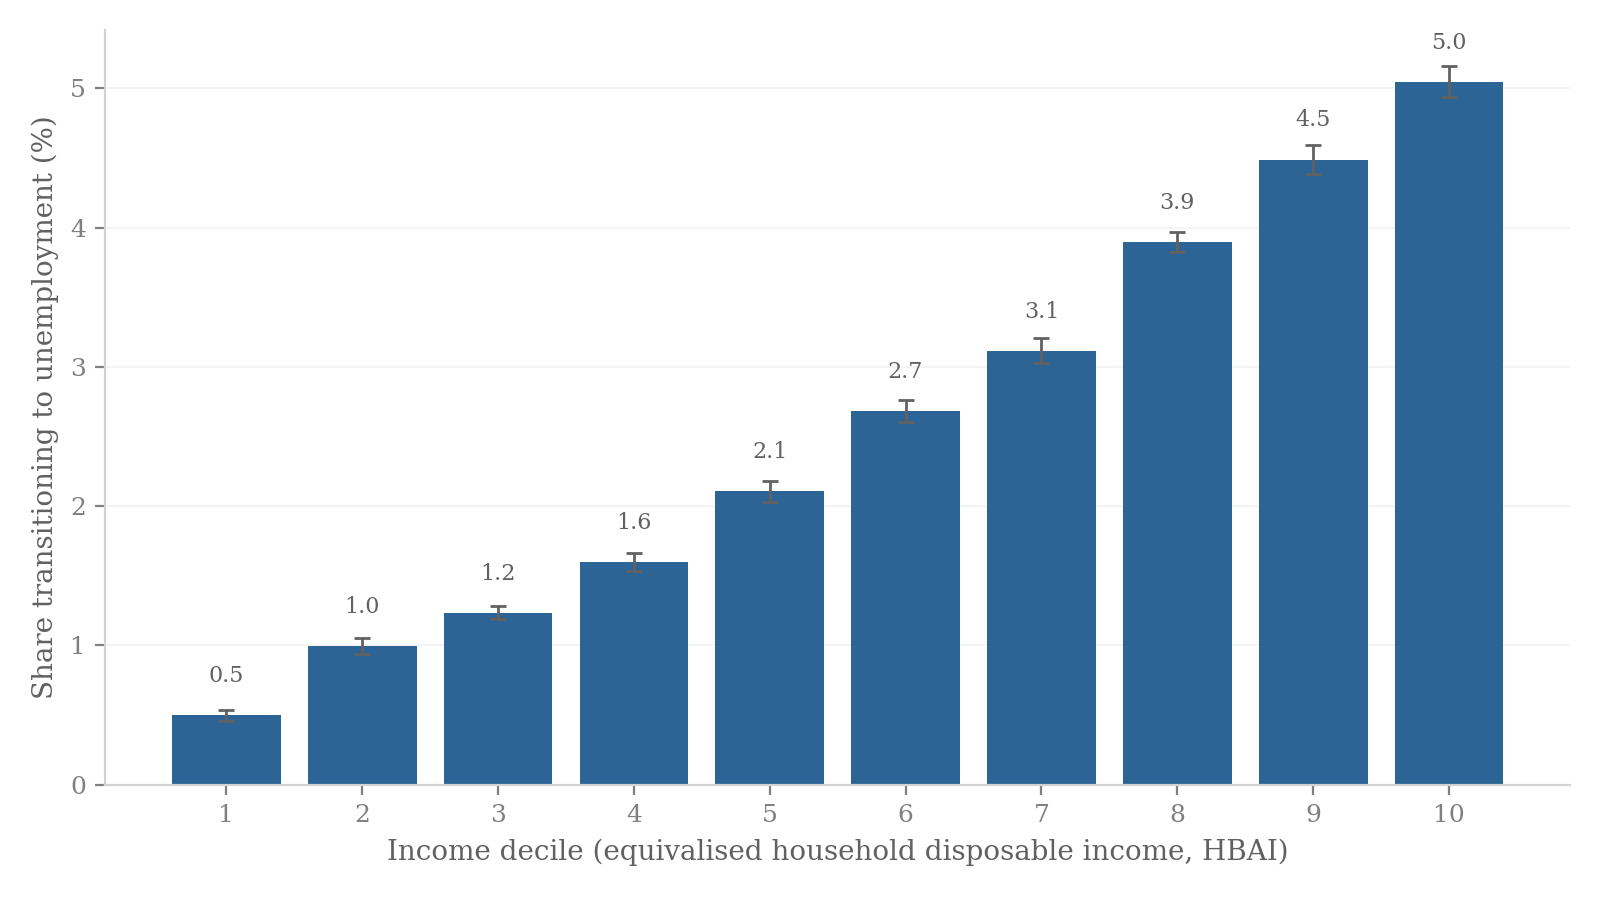
\includegraphics[width=.85\textwidth]{../results/jr16/fig4_1_transition.png}
\caption{Share of the population transitioning from employment to unemployment by equivalised disposable income decile, central scenario. Bars are means over 50 seeded displacement draws; error bars show central 95 per cent intervals across assignment draws. The gradient reflects the exposure-proportional allocation assumption, not observed incidence (see text).}
\label{fig:transition}
\end{figure}

The wage channel, by contrast, is almost distributionally flat. Figure~\ref{fig:wages} shows the percentage change in employment income among workers who remain employed: gains run from 2.50 per cent in the bottom decile to 2.72 per cent in the top, % results/jr16/fig4_2_wage_gain_by_decile.csv
a spread of barely 0.2 percentage points around the 2.6 per cent average uplift. Exposure is sufficiently widespread across the deciles in which people work that the productivity dividend is spread thinly and evenly. Under the central design, most cross-decile variation comes from the displacement margin. That allocation is a property of the scenario design rather than a finding: in the US evidence of \citet{acemoglu2022tasks}, task displacement operates chiefly through relative wage declines, which account for 50--70 per cent of changes in the wage structure. Section~\ref{sec:results-wagemargin} examines this alternative: a wage-margin implementation of the same headline calibration shifts losses from benefit caseloads to earnings, with a comparable fiscal cost but an almost entirely different poverty and inequality profile.

\begin{figure}[htbp]
\centering
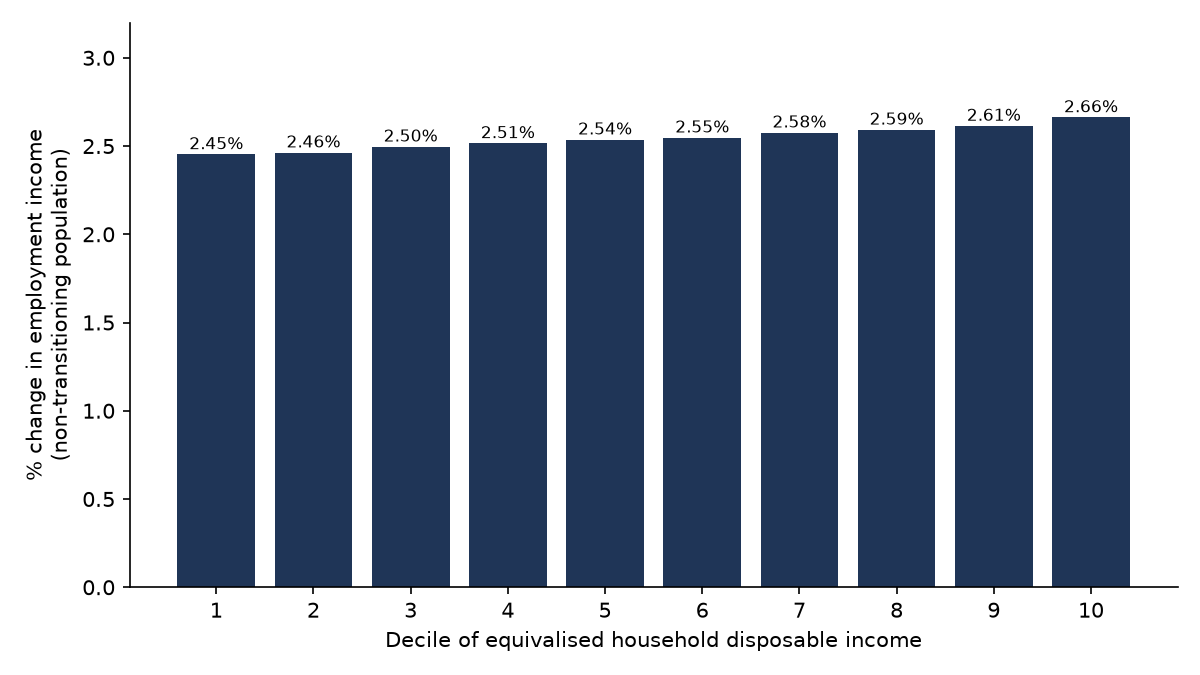
\includegraphics[width=.85\textwidth]{../results/jr16/fig4_2_wages.png}
\caption{Percentage change in employment income among workers remaining in employment, by income decile, central scenario. Means over 50 seeded draws.}
\label{fig:wages}
\end{figure}

The third channel is capital income. The scenario assumes part of the productivity gain is capitalised into returns on existing capital, applying a uniform proportional uplift to interest and dividend income (Section~\ref{sec:shocks}). Although the percentage change is identical across deciles by construction, Figure~\ref{fig:capital} shows the incidence in pounds is heavily concentrated: the top decile holds 35.2 per cent of all capital income (\pounds 8.1 billion of the baseline aggregate in my data), the top two deciles together more than half, and the bottom decile just 2.8 per cent. Under this proportional allocation, most simulated capital-income gains accrue to households already near the top of the distribution.

\begin{figure}[htbp]
\centering
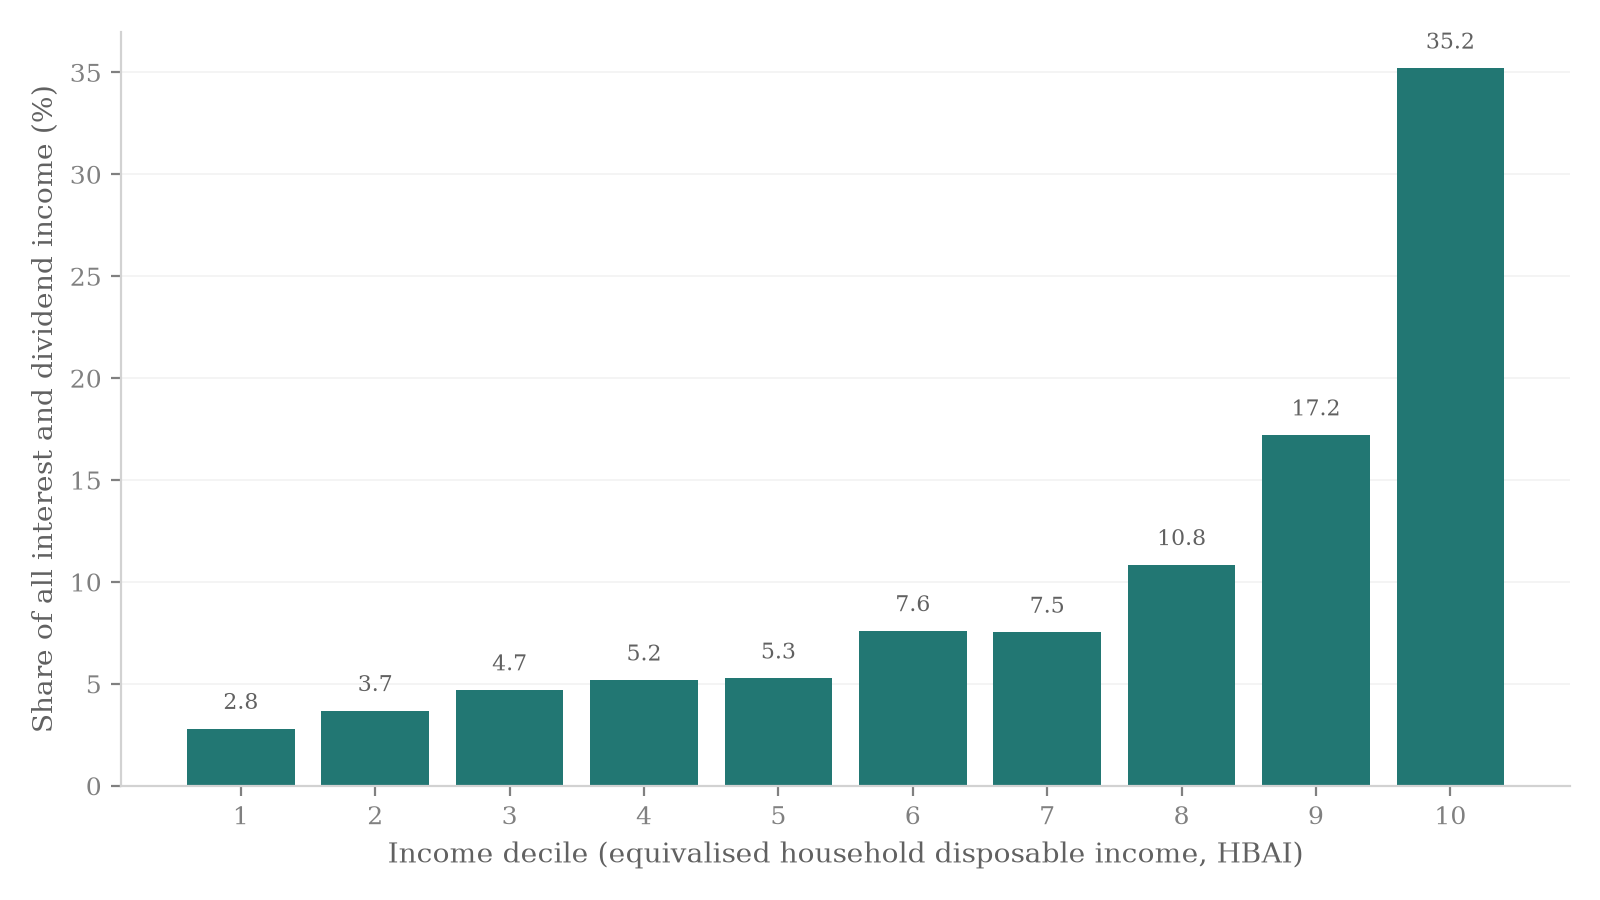
\includegraphics[width=.85\textwidth]{../results/jr16/fig4_3_capital.png}
\caption{Capital income channel by decile: a uniform proportional uplift, but pound gains concentrated where capital income is held.}
\label{fig:capital}
\end{figure}

\subsection{Household mediation of the shock}
\label{sec:results-mediation}

The tax-benefit system converts each market-income loss into a smaller disposable-income loss; Figure~\ref{fig:decomp} decomposes that mediation by decile into market income, benefits, and taxes and contributions, all expressed relative to baseline disposable income. The decomposition is household-level and additive: market income change plus benefit change minus tax change equals the disposable income change up to an explicit residual, which collects perimeter items inside the HBAI concept (council tax and pension deductions) and never exceeds 0.5 per cent of baseline income in any decile.

Market income losses follow the transition gradient: they are near zero in the bottom decile, around 0.8--2.0 per cent of baseline disposable income in deciles 3--5, between 3.3 and 4.1 per cent in deciles 7--9, and reach 6.7 per cent in the top decile. The tax-benefit system then cushions these losses through two distinct mechanisms. Across the middle deciles, automatic benefit entitlements---Universal Credit in particular---rise by up to 0.4 per cent of baseline income as displaced earners qualify for means-tested support. At the top the cushioning operates through the tax system instead: deciles 7--10 see their income tax and National Insurance liabilities fall by 0.4--2.0 per cent of baseline income as high-marginal-rate earnings disappear. The combined offset is substantial. In decile 10, a market income loss of 6.7 per cent of baseline disposable income becomes a disposable income loss of 4.3 per cent---roughly a third of the market shock absorbed---and in decile 5 a 1.8 per cent market loss becomes a 1.1 per cent disposable loss. Averaged over 20 displacement draws, disposable income losses run from 0.75 per cent in the bottom decile to 3.87 per cent in the top; the gradient is upward and stable across draws, though on the current 20-draw means it is not everywhere strictly monotone: decile 3 loses slightly less than decile 2 ($-0.85$ against $-0.93$ per cent) and deciles 9 and 10 are essentially tied ($-3.87$ per cent each), both differences well inside the draw noise. % seed-0 components from results/jr16/fig4_4_decomposition.csv; 20-draw means from results/appendix/decomposition_ci.csv

\begin{figure}[htbp]
\centering
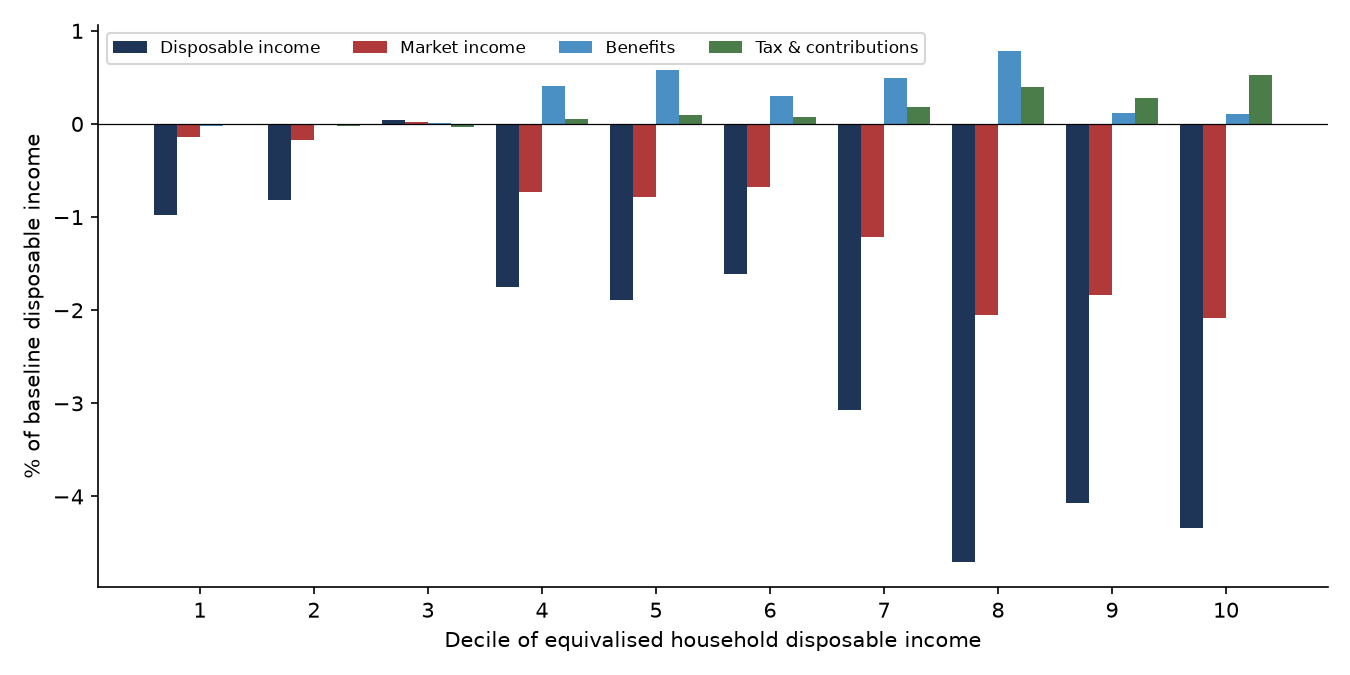
\includegraphics[width=.85\textwidth]{../results/jr16/fig4_4_decomposition.png}
\caption{Additive household-level decomposition of the change in income by decile into market income, benefits, and taxes and contributions, central scenario (single draw, seed 0), as a share of baseline HBAI disposable income. The residual collects perimeter items (council tax, pension deductions) inside the HBAI concept.}
\label{fig:decomp}
\end{figure}

\subsection{Fiscal and distributional aggregates}
\label{sec:results-aggregates}

Table~\ref{tab:presets} summarises the preset scenarios. In the central scenario the annual Exchequer cost is \pounds \genCentralCostBn~billion, driven by lost income tax and National Insurance on displaced higher earners together with higher benefit spending. Poverty rises by \genCentralPovBhcPp~percentage points before housing costs (\genCentralPovAhcPp~points after housing costs) and the Gini coefficient of equivalised disposable income rises by \genCentralGiniChangePp~percentage points from a baseline of \genBaselineGini. The low scenario---a 1 per cent displacement rate with no wage gain, which I treat purely as a sensitivity case rather than an estimate drawn from the literature---costs \pounds \genLowCostBn~billion and moves poverty and the Gini by roughly 0.2--0.3 points each. The high scenario, at 13 per cent displacement, costs \pounds \genHighCostBn~billion a year with poverty up \genHighPovBhcPp~points. PolicyEngine's before-housing-costs poverty line is an \emph{absolute} threshold, so these poverty changes measure absolute impoverishment rather than movement relative to a shock-shifted median. On the relative (60 per cent of contemporaneous median) BHC line the central scenario raises poverty by $+0.71 \pm 0.16$ percentage points over 50 draws --- well under half the absolute-line rise, because the shock lowers the median itself and so drags the relative line down with it. % results/robustness/central_monte_carlo.json relative_poverty_change_bhc_pp

The scenario anchors deserve a note of caution. The central calibration converts the task-exposure and productivity figures of \citet{briggs2023} into a displacement rate and a wage uplift via the conventions described in Section~\ref{sec:scenarios}; it is a calibration convention, not a forecast. The low scenario is likewise not an employment estimate from \citet{acemoglu2025}, whose 0.9--1.1 per cent figure refers to ten-year GDP growth, not job displacement.

\begin{table}[htbp]
\centering
\caption{Summary of preset scenarios (single draw, seed 0)}
\label{tab:presets}
\small
\begin{tabular}{lrrrr}
\toprule
Scenario & Displaced & Exchequer & $\Delta$ Poverty & $\Delta$ Gini \\
 & (million) & (\pounds bn/yr) & (BHC, pp) & (pp) \\
\midrule
Low & 0.24 & 4.3 & +0.33 & +0.21 \\
Central & 1.56 & 18.2 & +1.81 & +1.04 \\
High & 3.04 & 46.9 & +4.05 & +2.07 \\
% source: results/low.json, results/central.json, results/high.json (seed 0)
\bottomrule
\end{tabular}

\vspace{0.4em}
\parbox{0.92\textwidth}{\footnotesize\emph{Note:} Low: 1 per cent displacement, no wage gain (sensitivity case). Central: 7 per cent displacement, 2.6 per cent wage gain. High: 13 per cent displacement, 2.6 per cent wage gain. The capital-return shock (+0.4pp) applies in every preset.}
\end{table}

The central estimates are similar, but not identical, across the 50 assignment draws: the mean Exchequer cost is \pounds \genCentralMcCostMeanBn~billion (assignment-draw standard deviation \pounds \genCentralMcCostSdBn~billion; range \pounds \genCentralMcCostMinBn--\genCentralMcCostMaxBn~billion), with mean poverty and Gini increases of $\genCentralMcPovBhcMeanPp \pm \genCentralMcPovBhcSdPp$ and $\genCentralMcGiniMeanPp \pm \genCentralMcGiniSdPp$ percentage points. In the alternative indices tested, headline estimates change moderately: replacing C-AIOE with the DSIT AIOE mapping leaves the seed-0 Exchequer cost essentially unchanged, while the GPT-exposure measure of \citet{eloundou2023} raises it by about \pounds 2.2 billion (12 per cent); both produce similar upward transition gradients (Appendix~\ref{app:index-sensitivity}). % results/robustness/index_sensitivity_full.json

Two tested assumptions materially change the headline numbers. The first is displacement duration. The central scenario removes a full year of earnings from every displaced worker; under a 50 per cent earnings-retention hybrid---annual earnings are halved while employment status and hours remain those of full-year unemployment, so this approximates rather than models a six-month spell---the Exchequer cost falls from \pounds \genCentralMcCostMeanBn~billion to \pounds \genDurSixMoCostMeanBn~$\pm$~\genDurSixMoCostSdBn~billion and the BHC poverty rise all but vanishes ($+\genDurSixMoPovBhcMeanPp \pm \genDurSixMoPovBhcSdPp$ points), over 20 draws. The collapse is more than proportional---a na\"ive halving of the full-year result would give \pounds 8.9 billion---because workers who keep half a year's earnings remain taxpayers and largely stay clear of means-tested support. Every fiscal and poverty magnitude in this paper therefore scales strongly with the expected out-of-work duration, and the headline figures should be read as a full-year no-reemployment case. The second is benefit take-up. Imposing a 70 per cent Universal Credit take-up probability (drawn identically in baseline and shocked worlds) moves the cost to \pounds \genTakeupCostMeanBn~$\pm$~\genTakeupCostSdBn~billion and the poverty rise to $+\genTakeupPovBhcMeanPp \pm \genTakeupPovBhcSdPp$ points: the headline estimates change little under this single take-up sensitivity. % results/robustness/duration_takeup_sensitivity.json (variant half_earnings_retention; convex-combination comparator 8.86bn)

\subsection{The shock-size grid}
\label{sec:results-grid}

To move beyond the presets I simulate a grid of 66 scenarios, crossing eleven displacement rates (0 to 10 per cent of employees, allocated in proportion to exposure, as in the presets) with six wage uplifts (0 to 5 per cent), each combined with the capital income channel, all under exposure-proportional incidence. Figure~\ref{fig:griddisp} maps the change in average household disposable income. The corners bracket the range: with a 5 per cent wage gain and no job loss, average disposable income rises by 3.0 per cent; with 10 per cent displacement and no wage gain it falls by 5.1 per cent. % results/jr16/grid.csv
The near-zero contour runs close to the grid diagonal---at these calibrations, roughly one percentage point of wage growth offsets one percentage point of displacement in aggregate disposable income terms---so whether AI raises or lowers average living standards is highly sensitive, within this grid, to the balance struck between these two forces, about which the empirical literature remains genuinely uncertain.

\begin{figure}[htbp]
\centering
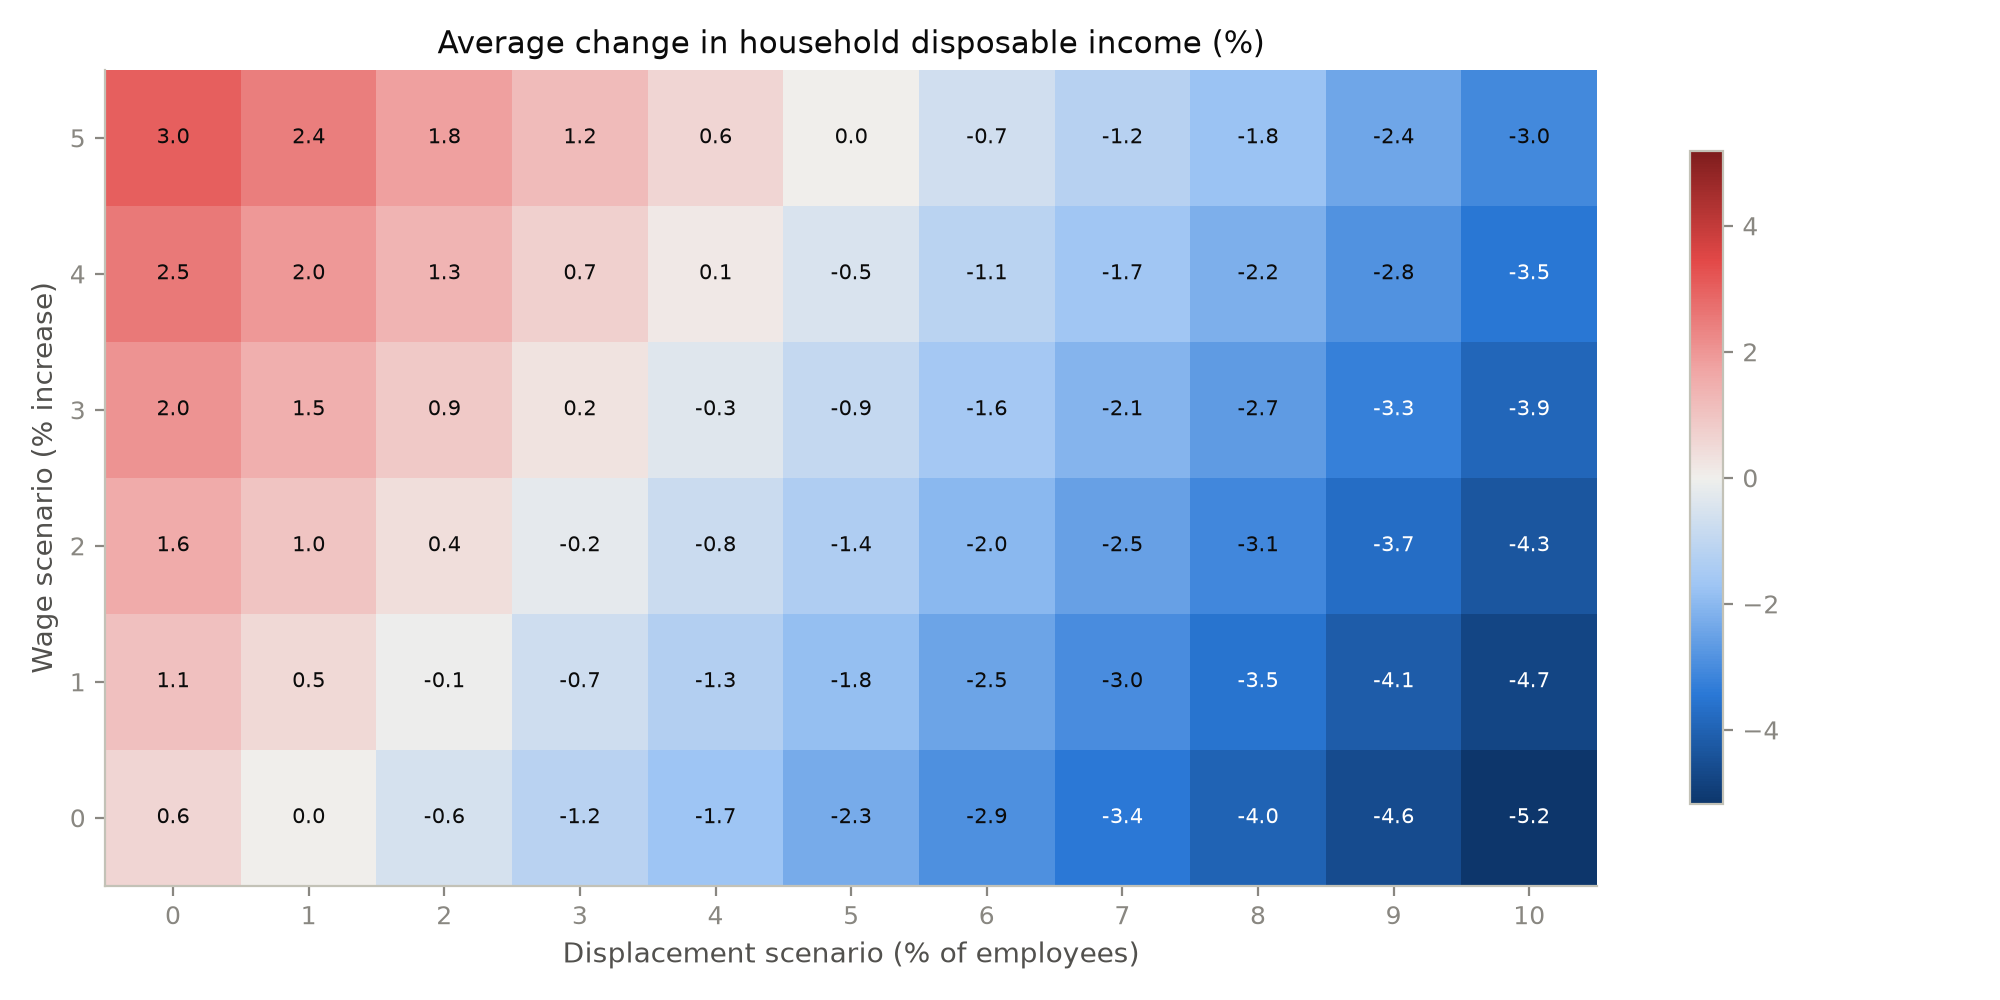
\includegraphics[width=.85\textwidth]{../results/jr16/fig4_5_disposable_grid.png}
\caption{Change in average household disposable income (per cent) across the 66-cell grid of displacement rates and wage uplifts (single draw, seed 0).}
\label{fig:griddisp}
\end{figure}

Figure~\ref{fig:gridrev} shows the corresponding fiscal picture. One measurement issue deserves note: in PolicyEngine's UK aggregates, income tax plus National Insurance minus total benefit expenditure (which includes the state pension) is a negative number, so expressing revenue changes relative to that net position produces uninformative percentages. I therefore express the net revenue change relative to gross income tax and National Insurance receipts as simulated on the household microdata (about \pounds 313 billion); this base is smaller than headline OBR receipts, which include employer contributions and income outside the household survey universe. Two consequences follow. First, the grid's revenue measure is income tax plus National Insurance minus cash benefit expenditure, a narrower concept than the full government-balance measure behind the \pounds \genCentralCostBn~billion headline cost of Section~\ref{sec:results-aggregates}, which also includes indirect taxes and other levies; the grid's cash-tax cost of the central 7 per cent/2.6 per cent scenario is roughly \pounds 11 billion (interpolated between the 2 and 3 per cent wage columns), and the two figures should not be read off the same surface. Second, on that narrower basis the grid spans a gain of \pounds 22.3 billion, or 7.2 per cent of receipts (5 per cent wage growth, no displacement), to a loss of \pounds 29.4 billion, or 9.4 per cent of receipts, in the worst cell (10 per cent displacement, no wage growth). At the central displacement rate, 7 per cent with no wage offset costs \pounds 21.2 billion (6.8 per cent of receipts), which a 3 per cent wage uplift more than halves to \pounds 9.8 billion. % results/jr16/grid.csv
As with disposable income, the break-even locus lies close to the diagonal.

\begin{figure}[htbp]
\centering
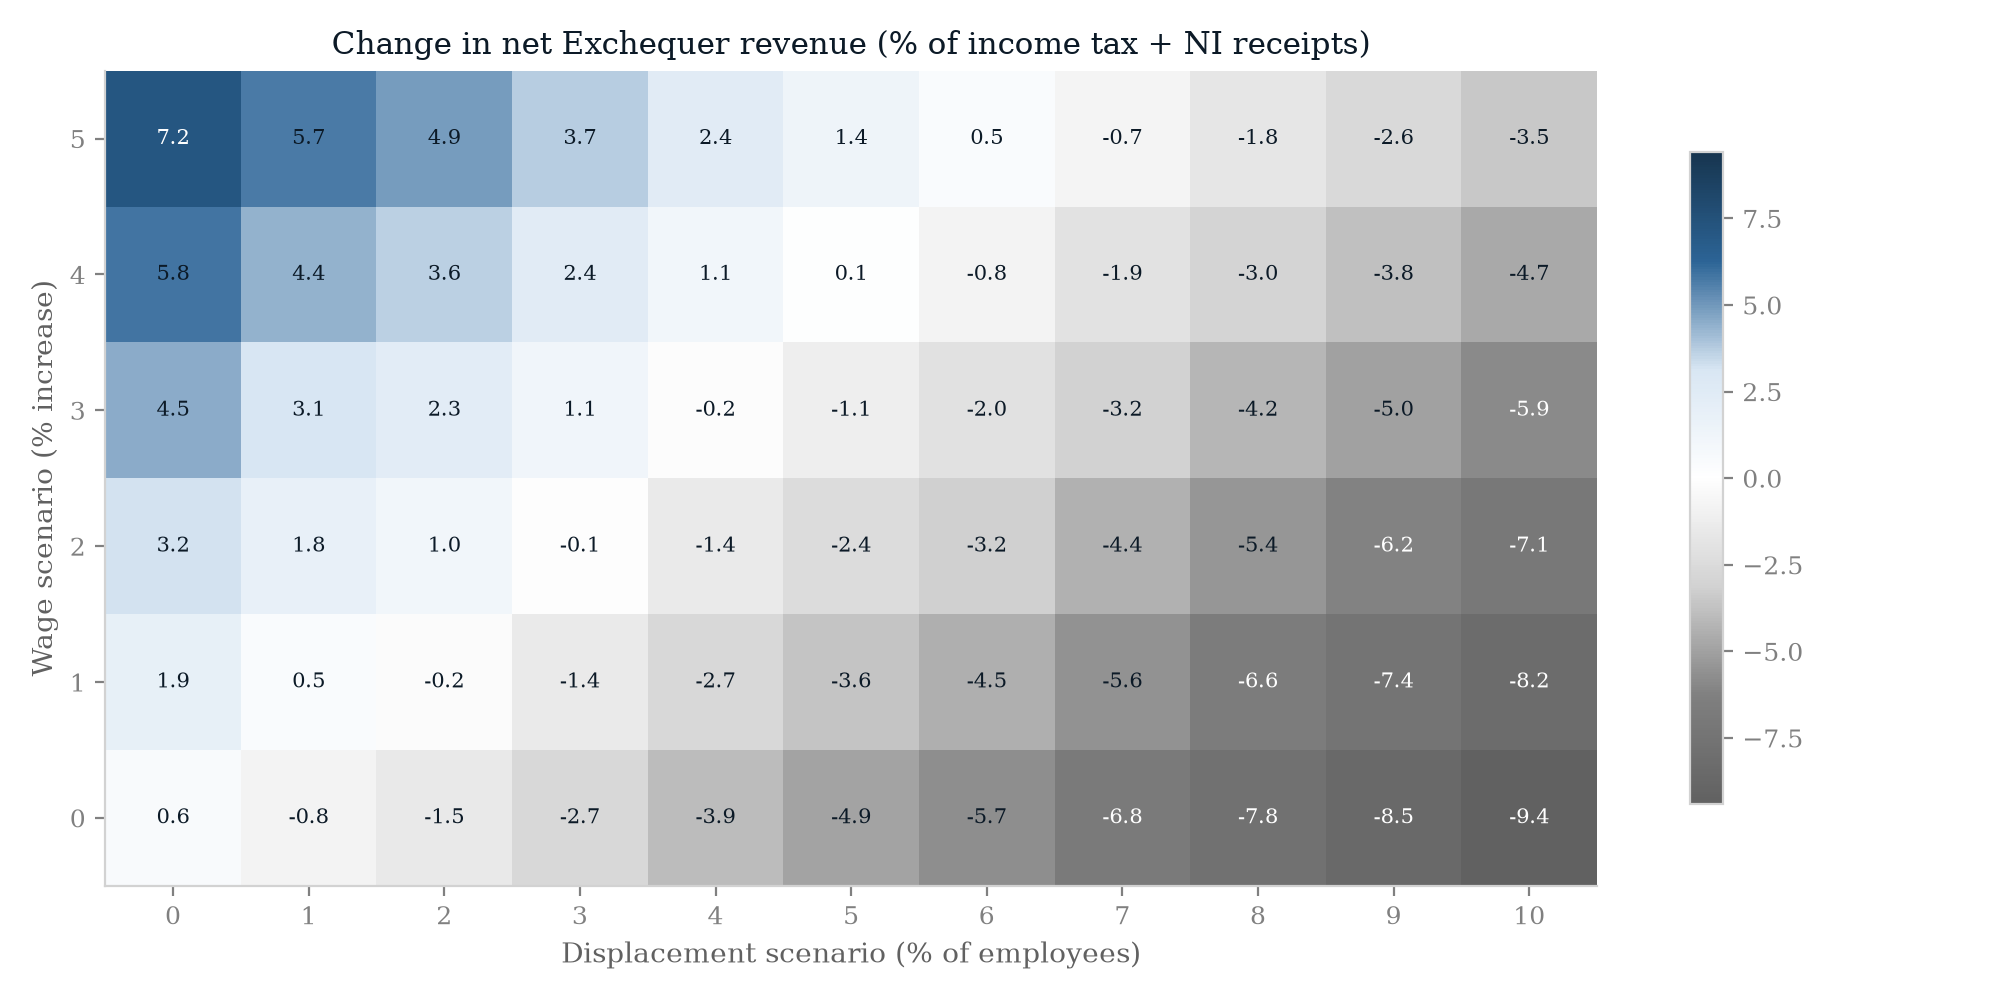
\includegraphics[width=.85\textwidth]{../results/jr16/fig4_6_exchequer_grid.png}
\caption{Net Exchequer revenue change as a percentage of gross income tax and National Insurance receipts, across the 66-cell scenario grid.}
\label{fig:gridrev}
\end{figure}

Figure~\ref{fig:gridgini} maps the change in the Gini coefficient across the same grid, and produces a consistent result within this grid: the Gini rises in all 66 cells, from +\genGridGiniMinPp{} percentage points in the capital-only cell (no displacement, no wage gain) to +\genGridGiniMaxPp{} points at the far corner. No combination of parameters within the grid reduces measured inequality. The simulated pattern is consistent with widening gaps at both ends of the distribution rather than a simple top-income gain, and it coexists with an incidence that is itself progressive: displacement strikes hardest at the top of the earnings ladder and pushes affected households down the distribution, while the wage uplift lifts the surviving employed---disproportionately in the upper-middle and top deciles---further away from workless and low-income households, and the capital channel reinforces the very top. Within the model, losses and gains are allocated in ways that widen gaps between households, and inequality rises even though the market shock lands mainly on higher earners.

\begin{figure}[htbp]
\centering
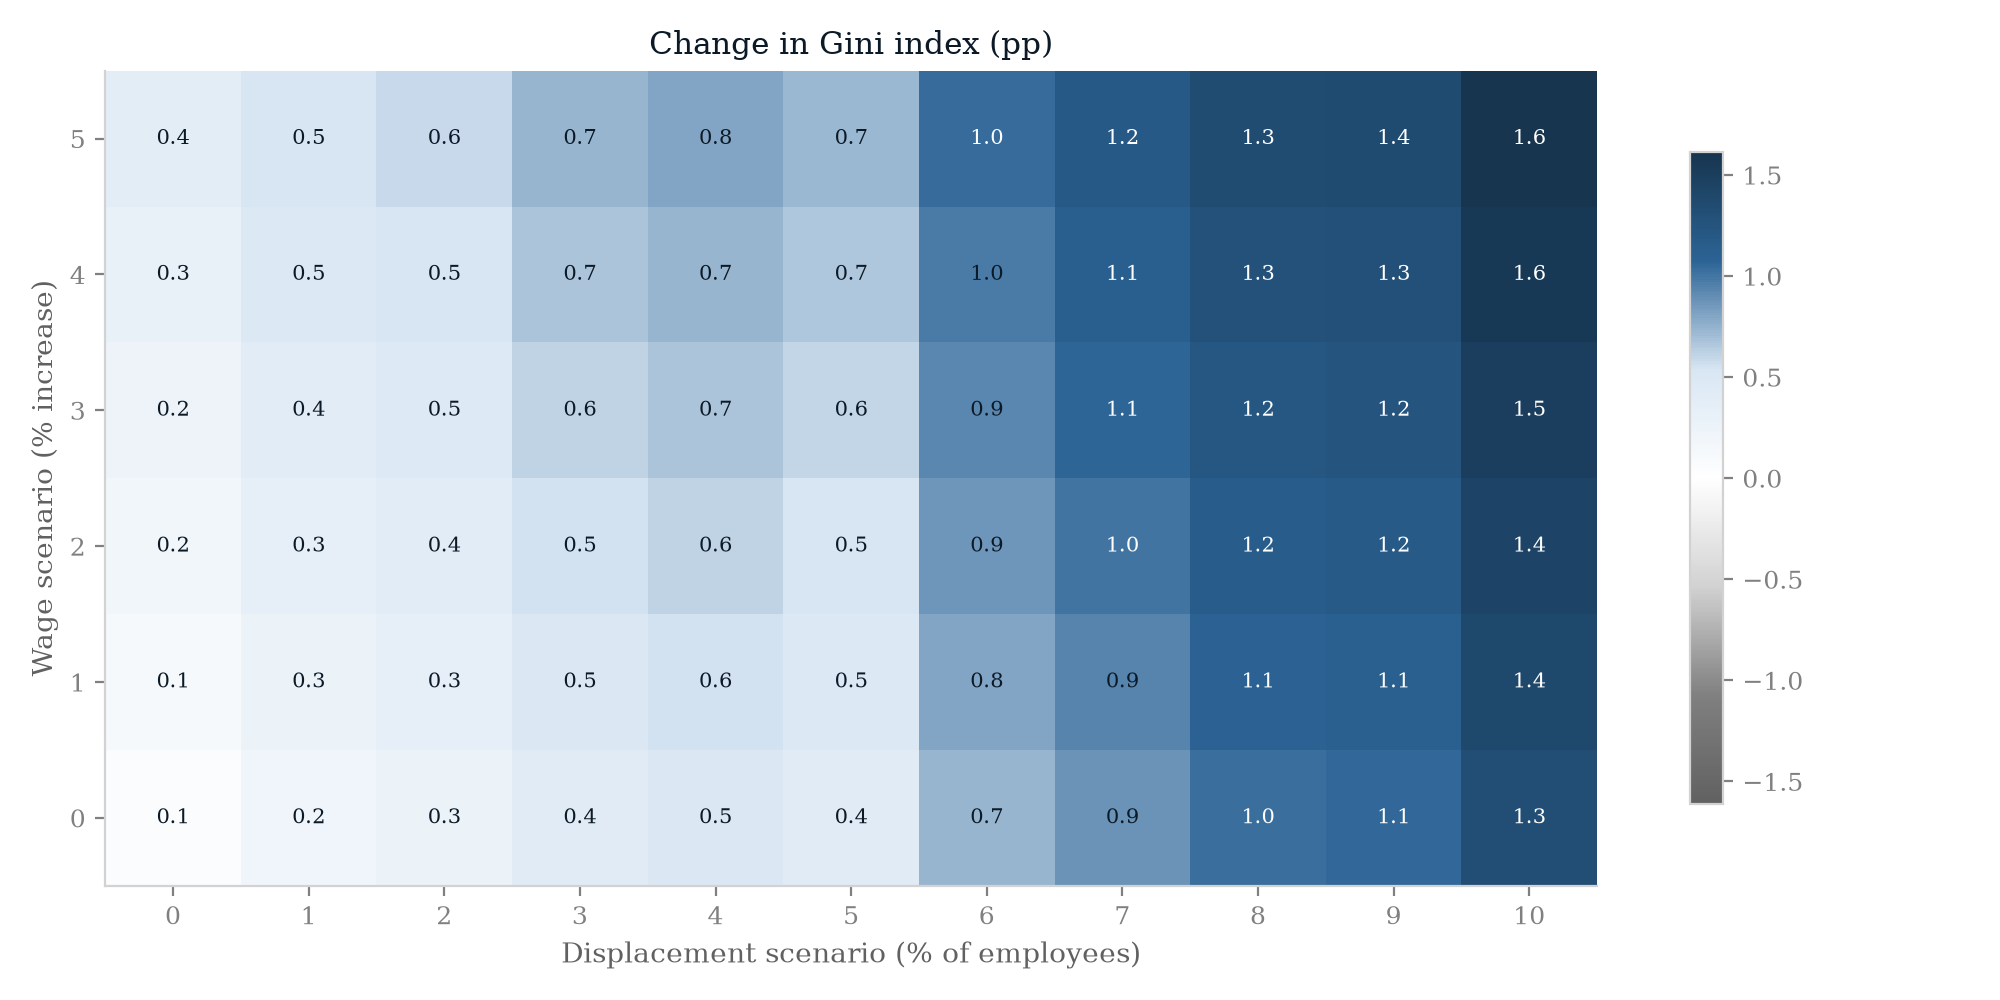
\includegraphics[width=.85\textwidth]{../results/jr16/fig4_7_gini_grid.png}
\caption{Change in the Gini coefficient of equivalised HBAI disposable income (percentage points) across the 66-cell scenario grid. The Gini rises in every cell.}
\label{fig:gridgini}
\end{figure}

\subsection{The incidence axis: who bears the shock}
\label{sec:results-incidence}

Everything so far conditions on exposure-proportional incidence. But allocation is at least as uncertain as shock size, so I reallocate the same central calibration across five families. Four are stylised: exposure-proportional, junior-concentrated, expertise-compression (implemented as a high-earner displacement tilt, not the \citet{hosseinilichtinger2026barriers} wage mechanism; Section~\ref{sec:incidence}) and uniform. The fifth is a Klein-anchored top-loaded stress test: exposure-proportional draws multiplied by an author-imposed junior tilt (1.29) and wage-tier tilt (9.6 above, 0.6 below median person earnings). Table~\ref{tab:incidence} gives means and assignment-draw standard deviations over 50 paired seeds.

\begin{table}[htbp]
\centering
\caption{Central shock under five incidence calibrations}
\label{tab:incidence}
\small
\setlength{\tabcolsep}{5pt}
\renewcommand{\arraystretch}{1.12}
\begin{tabular}{lrrrr}
\toprule
Incidence family & Displaced & Exchequer cost & $\Delta$ Poverty & $\Delta$ Gini \\
 & (million) & (\pounds bn/yr) & BHC (pp) & (pp) \\
\midrule
Exposure-proportional & 1.56 & 17.7 $\pm$ 1.2 & +1.87 $\pm$ 0.15 & +1.11 $\pm$ 0.09 \\
Junior-concentrated & 1.55 & 17.9 $\pm$ 1.6 & +1.85 $\pm$ 0.14 & +1.08 $\pm$ 0.08 \\
Expertise-compression & 1.67 & 20.6 $\pm$ 1.8 & +1.96 $\pm$ 0.15 & +1.04 $\pm$ 0.09 \\
Uniform & 1.55 & 13.9 $\pm$ 1.7 & +1.87 $\pm$ 0.17 & +1.16 $\pm$ 0.10 \\
Klein-anchored stress test & 1.62 & 32.8 $\pm$ 2.2 & +2.24 $\pm$ 0.14 & +0.97 $\pm$ 0.12 \\
% source: results/robustness/incidence_monte_carlo.json (means/sd); displaced from results/incidence/summary_five.csv (seed 0)
\bottomrule
\end{tabular}

\vspace{0.4em}
\parbox{0.92\textwidth}{\footnotesize\emph{Note:} Means $\pm$ assignment-draw standard deviations over 50 paired seeds. Assignment quantiles and Monte Carlo standard errors are reported separately in the machine-readable summary; they describe allocation noise, not population uncertainty. The Klein-anchored family combines exposure with author-imposed junior (1.29) and wage-tier (9.6 above / 0.6 below median person earnings) multipliers. The wage-tier values use press-release maximum-exposure scalings rather than the paper's per-standard-deviation estimates; this is a stress test, not an estimated displacement schedule. AHC poverty is evaluated on the same 50 draws as BHC poverty and the Gini.}
\end{table}

\begin{figure}[htbp]
\centering
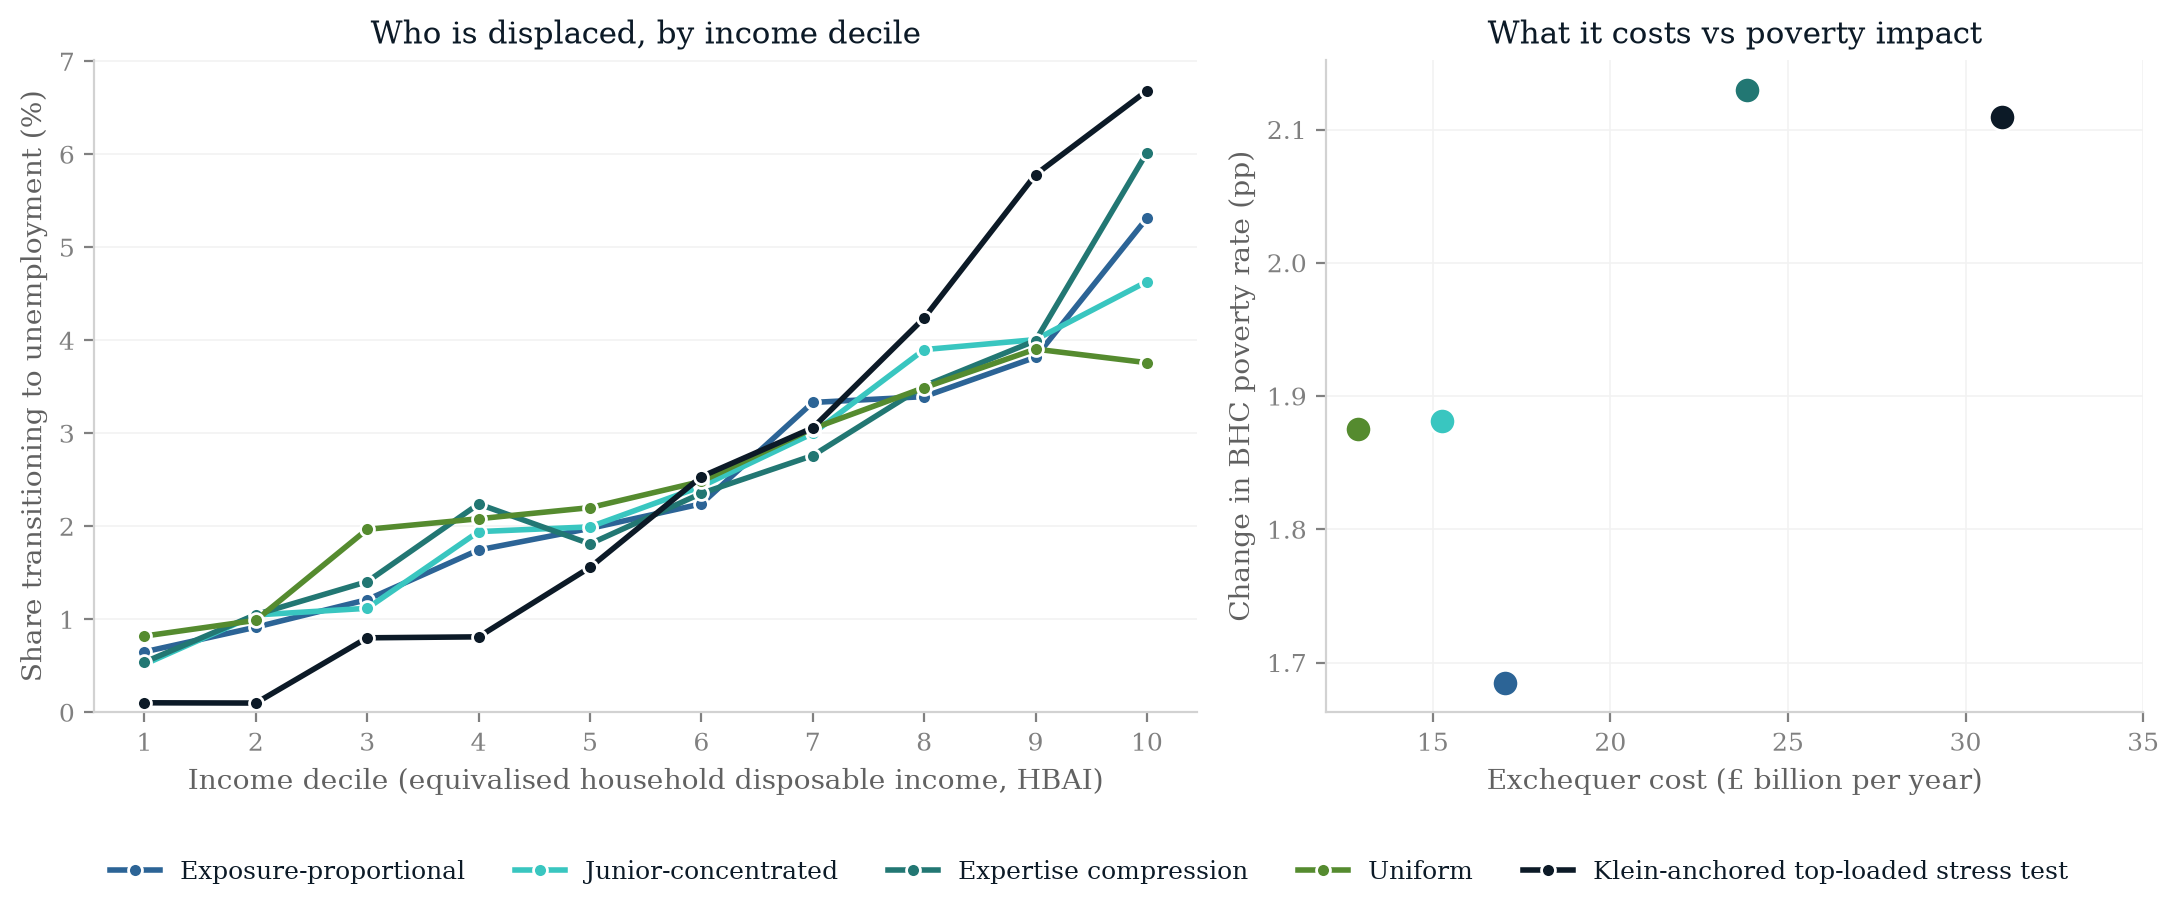
\includegraphics[width=.95\textwidth]{../results/incidence/incidence_families.png}
\caption{Decile incidence of the same aggregate central shock under five incidence families: share of each decile transitioning to unemployment, and change in equivalised HBAI disposable income by decile. The figure shows a single illustrative draw (seed 0), whereas the aggregates in Table~\ref{tab:incidence} are means over 50 Monte Carlo draws.}
\label{fig:incidence}
\end{figure}

Within these calibrations, who bears the shock materially changes its simulated cost. The mean Exchequer cost ranges from \pounds \genIncUniformCostMeanBn~billion under uniform incidence to \pounds \genIncKleinCostMeanBn~billion under the Klein-anchored stress test, generated by reallocating which workers lose their jobs. The larger fiscal effects under top-loaded incidence are consistent with the larger tax liabilities of the displaced high earners. These are paired-seed scenario comparisons, not population confidence statements.

% Paired 95% intervals recomputed from results/robustness/incidence_draws_five.csv (clean-room rebuild vintage; paired normal interval on draw-level differences, 50 shared seeds).
Across the four stylised families, the mean BHC poverty rise lies between \genIncFamilyPovBhcMeanMinPp{} and \genIncCompressionPovBhcMeanPp{} percentage points, while mean Exchequer costs span nearly \pounds 7 billion. Because the families share assignment seeds, draw-level \emph{differences} support paired inference: the expertise-compression poverty effect exceeds the exposure-proportional one by $+0.09$ points (paired 95 per cent interval $[+0.03, +0.15]$). The uniform--exposure poverty difference is indistinguishable from zero ($-0.00$ points, $[-0.06, +0.06]$); all families share the central wage and capital axis, so the comparison isolates displacement allocation. Uniform incidence retains a reliably smaller fiscal effect than exposure-proportional incidence ($-\pounds 3.84$ billion, $[-4.46, -3.21]$) alongside a reliably larger Gini effect (below). The junior-concentrated and exposure-proportional fiscal costs remain indistinguishable under the same paired comparison ($+\pounds 0.19$ billion, $[-\pounds 0.30, +\pounds 0.67]$). These paired intervals describe assignment-draw noise only, not population sampling uncertainty.

The author-imposed top-loaded calibrations combine relatively large fiscal and poverty effects. Expertise compression costs \pounds \genIncCompressionCostMeanBn~billion and raises BHC poverty by +\genIncCompressionPovBhcMeanPp{} points. The Klein-anchored stress test has means of \pounds 32.8 billion and +2.24 points; its AHC effect is evaluated over the same 50 assignment draws. Its wage-tier multiplier produces the most top-tilted seed-0 gradient, from 0.01 per cent transitioning in the bottom decile to 7.25 per cent in the top. These magnitudes are conditional on the stress-test mapping and are not estimates transported from Klein Teeselink.

The Gini rises in all five simulated families---50-draw means of +\genIncFamilyGiniMeanMinPp{} to +\genIncFamilyGiniMeanMaxPp{} percentage points---just as it rises in all 66 grid cells (in the appendix's capital-off variant of the grid the null cell with no shock at all is exactly zero, as it must be). Paired inference again separates some families: the uniform Gini effect exceeds the exposure-proportional one by $+0.04$ points (paired 95 per cent interval $[+0.01, +0.08]$), and the Klein-anchored Gini effect is reliably \emph{smaller} than the expertise-compression one ($-0.07$ points, $[-0.12, -0.03]$), consistent with its more top-concentrated losses compressing the upper tail. % paired intervals from results/robustness/incidence_draws_five.csv (50 shared seeds)
The directional result is explicitly conditional on these displacement calibrations.

\subsection{The adjustment margin: wage cuts versus displacement}
\label{sec:results-wagemargin}

The incidence families reallocate displacement across workers; the wage-margin family instead moves the same shock to the wage margin. Every employee keeps their job, and earnings are removed through author-imposed occupation-level cuts proportional to C-AIOE or PSS, calibrated so that the aggregate employee-earnings loss equals the realised gross earnings loss of the paired central displacement draw---7.77 per cent of the baseline wage bill at seed 0 (recorded target share 0.07774), larger than the 7 per cent head-count rate because group job-loss rates correlate with group pay; the equality is asserted in code. The PSS rows are a PSS-ranked wage-cut stress test, not the \citet{hosseinilichtinger2026barriers} labour-supply mechanism. Table~\ref{tab:wagemargin} compares these clearly labelled calibrations on the seed-0 basis. % results/wage_margin_central.json gross_cut_share_target = 0.07773605...

\begin{table}[htbp]
\centering
\caption{The headline calibration on two adjustment margins (central calibration; displacement row single draw, seed 0; wage-margin rows deterministic)}
\label{tab:wagemargin}
\small
\begin{tabular}{lrrr}
\toprule
Scenario & Exchequer cost & $\Delta$ Poverty & $\Delta$ Gini \\
 & (\pounds bn/yr) & BHC (pp) & (pp) \\
\midrule
Central displacement & 18.2 & +1.81 & +1.04 \\
Wage margin (C-AIOE gradient) & 26.6 & +0.10 & $-$0.44 \\
Wage margin (PSS gradient) & 26.4 & +0.17 & $-$0.35 \\
% source: results/central.json, results/wage_margin_central.json, results/wage_margin_pss.json
\bottomrule
\end{tabular}

\vspace{0.4em}
\parbox{0.92\textwidth}{\footnotesize\emph{Note:} The wage-margin rows remove the same aggregate gross earnings as the paired seed-0 central displacement draw (7.77 per cent of the baseline employee wage bill); the displacement row removes the earnings of a weighted 7 per cent of employees. All rows apply the 2.6 per cent wage uplift and the capital shock. The wage-margin scenarios displace no one: cuts are occupation-level percentages proportional to the stated gradient, calibrated to the stated baseline-wage-bill share. After-housing-costs poverty changes are +1.85, +0.27 and +0.35 points respectively.}
\end{table}

Three contrasts stand out. First, under the simulated wage schedules the fiscal cost rises from \pounds \genCentralCostBn~billion to \pounds \genWageMarginCentralCostBn~billion (\pounds \genWageMarginPssCostBn~billion under the PSS gradient). Wage cuts shave earnings at marginal tax and National Insurance rates, whereas displacement removes whole earnings blocks and is partly offset by means-tested benefits. This comparison is conditional on these calibrations and does not establish a general lower bound.

Second, the poverty effect all but disappears in the simulated wage-cut cases: the +1.81-point BHC poverty rise becomes +0.10 points under the C-AIOE gradient and +0.17 under PSS. Spreading the calibrated loss across employees pushes fewer households across the frozen absolute line than concentrating losses on displaced workers; this does not establish a bound for other wage schedules.

Third, the sign of the inequality effect flips under both author-chosen wage gradients: the Gini falls by 0.44 and 0.35 points, whereas it rises in the simulated displacement cells. Percentage cuts scale with gradients concentrated in well-paid occupations, compressing earnings from above. The comparison shows that poverty and inequality conclusions depend on both the adjustment margin and its imposed schedule; it does not establish a universal fiscal or distributional result.

Table~\ref{tab:mixedwage} makes the like-for-like comparison. In every row gross earnings loss before the common uplift is 7.77 per cent of the baseline wage bill, exactly the loss realised in the seed-0 central/exposure draw to which the exercise is paired. Moving that fixed loss from wage cuts to displacement reduces the Exchequer cost from \pounds 26.6 billion to \pounds 18.2 billion, while raising BHC poverty from 0.10 to 1.81 points and the Gini effect from $-0.44$ to $+1.04$ points. The half-index case costs \pounds 22.7 billion, raises poverty by 1.02 points and raises the Gini by 0.29 points. Net employee-income losses after the uplift rise slightly, from 5.11 to 5.32 per cent, because fewer survivors receive the uplift as displacement rises; the pre-uplift loss being compared is invariant. % results/robustness/mixed_adjustment.csv
Conditional on this author-designed allocation rule, the monotone poverty and inequality patterns track the shifting adjustment margin; they are not structural causal estimates.

\begin{table}[htbp]
\centering
\caption{Adjustment-margin and survivor-wage sensitivities (seed 0, 2026)}
\label{tab:mixedwage}
\small
\begin{tabular}{lrrrr}
\toprule
Scenario & Displaced & Exchequer cost & $\Delta$ Poverty & $\Delta$ Gini \\
 & (million) & (\pounds bn/yr) & BHC (pp) & (pp) \\
\midrule
\multicolumn{5}{l}{\emph{Fixed gross earnings loss (7.77 per cent); $\lambda$ scales displacement}} \\
$\lambda=0$ & 0.00 & 26.6 & +0.10 & $-$0.44 \\
$\lambda=.25$ & 0.42 & 24.5 & +0.61 & $-$0.03 \\
$\lambda=.50$ & 0.77 & 22.7 & +1.02 & +0.29 \\
$\lambda=.75$ & 1.15 & 20.6 & +1.39 & +0.62 \\
$\lambda=1$ & 1.56 & 18.2 & +1.81 & +1.04 \\
\midrule
\multicolumn{5}{l}{\emph{Central 7 per cent displacement with alternative survivor-wage effects}} \\
$-5.0\%$ & 1.56 & 57.3 & +2.65 & +0.59 \\
$-2.6\%$ & 1.56 & 45.0 & +2.21 & +0.73 \\
$0.0\%$ & 1.56 & 31.6 & +2.01 & +0.88 \\
$+2.6\%$ & 1.56 & 18.2 & +1.81 & +1.04 \\
$+5.0\%$ & 1.56 & 5.8 & +1.68 & +1.19 \\
% source: results/robustness/mixed_adjustment.csv, results/robustness/survivor_wage_grid.csv
\bottomrule
\end{tabular}

\vspace{0.4em}
\parbox{0.92\textwidth}{\footnotesize\emph{Note:} In the mixed panel, $\lambda$ thins the central 7 per cent employee-displacement draw and C-AIOE-graded survivor cuts fill the gap to that same seed-0 draw's gross pre-uplift earnings loss (7.77 per cent of the wage bill). Gross loss is identical in every row; the 2.6 per cent complementarity-graded uplift and capital shock then apply. The pure wage-cut endpoint therefore matches the C-AIOE wage-margin row's gross-loss calibration. The second panel holds displaced workers and the capital shock fixed and changes only the employment-weighted survivor-wage parameter. These are author-designed reduced-form comparative statics, not estimates of equilibrium wage responses.}
\end{table}

Allowing survivor wages to fall is more consequential for the level of the fiscal estimate. With the same 1.56 million displaced workers, removing the productivity pass-through raises the Exchequer cost from \pounds 18.2 billion to \pounds 31.6 billion; an average 2.6 per cent wage decline raises it to \pounds 45.0 billion, and a 5 per cent decline to \pounds 57.3 billion. Poverty also rises, but less dramatically, from 1.81 points under the central uplift to 2.65 points under a 5 per cent wage decline, because the additional loss is spread across survivors rather than concentrated as total earnings loss. The assumed positive wage pass-through is a large fiscal offset in this grid. The Gini remains positive in every central-displacement wage cell, including the adverse-wage cases; more positive survivor gains are associated with a larger Gini response, consistent with a wider gap between displaced workers and those who keep their jobs.

\subsection{The age and gender dimensions}
\label{sec:results-agegender}

The incidence axis has a within-family age structure worth drawing out. Under exposure-proportional incidence, workers aged 16--24 account for only 5.3 per cent of the displaced in the central scenario, because young people in the UK are concentrated in low-exposure service occupations; the burden falls on prime-age workers (27.1 per cent of the displaced are aged 35--44). The junior-concentrated family of Table~\ref{tab:incidence} reweights displacement probabilities towards junior workers while holding the aggregate displacement rate at 7 per cent; because juniors are concentrated in occupation groups whose fixed quotas the tilt does not change, the realised seed-0 age composition barely moves (a 16--24 share of 4.8 per cent and a 55--64 share of 18.3 against 18.1 per cent), and the aggregate differences are small relative to variation across the 50 assignment draws for cost (\pounds 17.9 $\pm$ 1.6 under the junior tilt against \pounds 17.7 $\pm$ 1.2 billion under exposure-proportional incidence), poverty and the Gini alike. The exercise shows that the junior tilt is an additional scenario assumption rather than a consequence of occupational exposure alone---and that, within fixed occupation quotas, it does little to redirect the shock towards the young. Even under the junior tilt, prime-age workers remain the largest displaced group. % age shares: results/central.json, results/central_youth_tilted.json (seed 0)

If AI adoption in practice falls hardest on juniors through recruitment rather than dismissal---as the seniority-biased hiring evidence of \citet{hosseini2026} and the early-career employment declines in AI-exposed occupations documented by \citet{brynjolfsson2025} suggest---the fiscal consequences could differ materially from the broad-based scenarios above, because junior workers contribute little income tax and National Insurance. That channel, however, operates through hiring flows that stock-based simulation frameworks such as mine do not capture by construction.

Exposure also carries a gender gradient. Employed women in the FRS have a mean C-AIOE of 0.33 against 0.18 for employed men, reflecting women's concentration in administrative, professional and associate-professional work. In the central scenario this translates into a displacement rate of 7.5 per cent for employed women against 6.5 per cent for men (means over 20 draws): women hold 51.8 per cent of employment but account for 55.4 per cent of the displaced. Household-level income changes are nevertheless similar by sex ($-2.9$ per cent for both women and men). % results/appendix/gender_incidence.json
A natural reading is that income pooling within couples mutes the individual asymmetry at the household level, though I have not decomposed the result and offer this as a hypothesis rather than a finding. The individual-level asymmetry itself echoes the international evidence that female employment is substantially more exposed to generative AI than male employment \citep{ilo2025}.

\subsection{Benefit caseloads}
\label{sec:results-caseloads}

The fiscal aggregates above can also be read on the delivery side, as caseloads. In the central scenario the shock draws 370,000 benefit units into Universal Credit while 59,000 exit, a net caseload increase of \genCaseloadNetNewUcBenunitsK,000 benefit units, and annual UC spending rises by \pounds \genCaseloadUcSpendChangeBn~billion from a baseline of \pounds 41.4 billion, of which \pounds 0.4 billion is the housing element within paid awards. Against DWP's roughly \pounds 334 billion of welfare spending in 2025--26 (a context figure, not a model output), the central increment is about 1 per cent; the high scenario roughly doubles it (674,000 net new benefit units, +\pounds 6.3 billion), while the low scenario adds only 30,000 benefit units and \pounds 0.3 billion. Caseload responses vary with incidence in the expected direction: the junior-concentrated family, whose displaced workers more often live in households with other earners, adds fewer benefit units (251,000 net) at lower cost (+\pounds 2.4 billion). Two accounting notes apply: only the benefit-unit figures are net of exits---the corresponding household and person counts (353,000 and \genCaseloadNewUcPersonsK,000 in the central scenario) are gross new entrants---and the housing element is measured within paid awards, slightly overstating housing-specific cash. % results/caseloads/summary.csv
